
%\documentclass[11pts,a4paper,amsmath,amssymb,floatfix]{article}%{report}%{book}
\documentclass[12pts,a4paper,amsmath,amssymb,floatfix]{article}%{report}%{book}
\usepackage{graphicx}
\usepackage{wrapfig,pdfpages}% Include figure files
%\usepackage{dcolumn,enumerate}% Align table columns on decimal point
\usepackage{enumerate}%,enumitem}% Align table columns on decimal point
\usepackage{bm,dpfloat}% bold math
%\usepackage[pdftex,bookmarks,colorlinks=true,urlcolor=rltblue,citecolor=blue]{hyperref}
\usepackage{amsfonts,amsmath,amssymb,stmaryrd,indentfirst}
\usepackage{times,psfrag}
\usepackage{natbib}
\usepackage{color}
\usepackage{units}
\usepackage{rotating}
\usepackage{multirow}


\usepackage{pifont}
\usepackage{subfigure}
\usepackage{subeqnarray}
\usepackage{ifthen}

\usepackage{supertabular}
\usepackage{moreverb}
\usepackage{listings}
\usepackage{palatino}
%\usepackage{doi}
\usepackage{longtable}
\usepackage{float}
\usepackage{perpage}
\MakeSorted{figure}
%\usepackage{pdflscape}
\usepackage{soul} %% use \hl to higlight text

\usepackage{framed}
\definecolor{shadecolor}{gray}{0.9}
%\usepackage{booktabs}
%\newcommand{\ra}[1]{\renewcommand{\arraystretch}{#1}}


\definecolor{rltblue}{rgb}{0,0,0.75}


%\usepackage{natbib}
\usepackage{fancyhdr} %%%%
\pagestyle{fancy}%%%%
% with this we ensure that the chapter and section
% headings are in lowercase
%%%%\renewcommand{\chaptermark}[1]{\markboth{#1}{}}
\renewcommand{\sectionmark}[1]{\markright{\thesection\ #1}}
\fancyhf{} %delete the current section for header and footer
\fancyhead[LE,RO]{\bfseries\thepage}
\fancyhead[LO]{\bfseries\rightmark}
\fancyhead[RE]{\bfseries\leftmark}
\renewcommand{\headrulewidth}{0.5pt}
% make space for the rule
\fancypagestyle{plain}{%
\fancyhead{} %get rid of the headers on plain pages
\renewcommand{\headrulewidth}{0pt} % and the line
}

\def\newblock{\hskip .11em plus .33em minus .07em}
\usepackage{color}

%\usepackage{makeidx}
%\makeindex

\setlength\textwidth      {16.cm}
\setlength\textheight     {22.6cm}
\setlength\oddsidemargin  {-0.3cm}
\setlength\evensidemargin {0.3cm}

\setlength\headheight{14.49998pt}
\setlength\topmargin{0.0cm}
\setlength\headsep{1.cm}
\setlength\footskip{1.cm}
\setlength\parskip{0pt}
\setlength\parindent{0pt}


%%%
%%% Headers and Footers
\lhead[] {\text{\small{EG501V -- Computational Fluid Dynamics}}}
\rhead[\text{\small{Assignment 2016/17}}]{Assignment 2016/17}
%\rfoot[] {{\text{\small{EOS + Mass Conservation using Matlab }}}}
%\chead[] {\text{\small{Session 2012/13}}}
\lfoot[]{CFD}
\rfoot[\thepage]{\thepage}
\renewcommand{\headrulewidth}{0.8pt}


%%%
%%% space between lines
%%%
\renewcommand{\baselinestretch}{1.5}

\newenvironment{VarDescription}[1]%
  {\begin{list}{}{\renewcommand{\makelabel}[1]{\textbf{##1:}\hfil}%
    \settowidth{\labelwidth}{\textbf{#1:}}%
    \setlength{\leftmargin}{\labelwidth}\addtolength{\leftmargin}{\labelsep}}}%
  {\end{list}}

%%%%%%%%%%%%%%%%%%%%%%%%%%%%%%%%%%%%%%%%%%%
%%%%%%                              %%%%%%%
%%%%%%      NOTATION SECTION        %%%%%%%
%%%%%%                              %%%%%%%
%%%%%%%%%%%%%%%%%%%%%%%%%%%%%%%%%%%%%%%%%%%

% Text abbreviations.
\newcommand{\ie}{{\em{i.e., }}}
\newcommand{\eg}{{\em{e.g., }}}
\newcommand{\cf}{{\em{cf., }}}
\newcommand{\wrt}{with respect to}
\newcommand{\lhs}{left hand side}
\newcommand{\rhs}{right hand side}
% Commands definining mathematical notation.

% This is for quantities which are physically vectors.
\renewcommand{\vec}[1]{{\mbox{\boldmath$#1$}}}
% Physical rank 2 tensors
\newcommand{\tensor}[1]{\overline{\overline{#1}}}
% This is for vectors formed of the value of a quantity at each node.
\newcommand{\dvec}[1]{\underline{#1}}
% This is for matrices in the discrete system.
\newcommand{\mat}[1]{\mathrm{#1}}


\DeclareMathOperator{\sgn}{sgn}
\newtheorem{thm}{Theorem}[section]
\newtheorem{lemma}[thm]{Lemma}

%\newcommand\qed{\hfill\mbox{$\Box$}}
\newcommand{\re}{{\mathrm{I}\hspace{-0.2em}\mathrm{R}}}
\newcommand{\inner}[2]{\langle#1,#2\rangle}
\renewcommand\leq{\leqslant}
\renewcommand\geq{\geqslant}
\renewcommand\le{\leqslant}
\renewcommand\ge{\geqslant}
\renewcommand\epsilon{\varepsilon}
\newcommand\eps{\varepsilon}
\renewcommand\phi{\varphi}
\newcommand{\bmF}{\vec{F}}
\newcommand{\bmphi}{\vec{\phi}}
\newcommand{\bmn}{\vec{n}}
\newcommand{\bmns}{{\textrm{\scriptsize{\boldmath $n$}}}}
\newcommand{\bmi}{\vec{i}}
\newcommand{\bmj}{\vec{j}}
\newcommand{\bmk}{\vec{k}}
\newcommand{\bmx}{\vec{x}}
\newcommand{\bmu}{\vec{u}}
\newcommand{\bmv}{\vec{v}}
\newcommand{\bmr}{\vec{r}}
\newcommand{\bma}{\vec{a}}
\newcommand{\bmg}{\vec{g}}
\newcommand{\bmU}{\vec{U}}
\newcommand{\bmI}{\vec{I}}
\newcommand{\bmq}{\vec{q}}
\newcommand{\bmT}{\vec{T}}
\newcommand{\bmM}{\vec{M}}
\newcommand{\bmtau}{\vec{\tau}}
\newcommand{\bmOmega}{\vec{\Omega}}
\newcommand{\pp}{\partial}
\newcommand{\kaptens}{\tensor{\kappa}}
\newcommand{\tautens}{\tensor{\tau}}
\newcommand{\sigtens}{\tensor{\sigma}}
\newcommand{\etens}{\tensor{\dot\epsilon}}
\newcommand{\ktens}{\tensor{k}}
\newcommand{\half}{{\textstyle \frac{1}{2}}}
\newcommand{\tote}{E}
\newcommand{\inte}{e}
\newcommand{\strt}{\dot\epsilon}
\newcommand{\modu}{|\bmu|}
% Derivatives
\renewcommand{\d}{\mathrm{d}}
\newcommand{\D}{\mathrm{D}}
\newcommand{\ddx}[2][x]{\frac{\d#2}{\d#1}}
\newcommand{\ddxx}[2][x]{\frac{\d^2#2}{\d#1^2}}
\newcommand{\ddt}[2][t]{\frac{\d#2}{\d#1}}
\newcommand{\ddtt}[2][t]{\frac{\d^2#2}{\d#1^2}}
\newcommand{\ppx}[2][x]{\frac{\partial#2}{\partial#1}}
\newcommand{\ppxx}[2][x]{\frac{\partial^2#2}{\partial#1^2}}
\newcommand{\ppt}[2][t]{\frac{\partial#2}{\partial#1}}
\newcommand{\pptt}[2][t]{\frac{\partial^2#2}{\partial#1^2}}
\newcommand{\DDx}[2][x]{\frac{\D#2}{\D#1}}
\newcommand{\DDxx}[2][x]{\frac{\D^2#2}{\D#1^2}}
\newcommand{\DDt}[2][t]{\frac{\D#2}{\D#1}}
\newcommand{\DDtt}[2][t]{\frac{\D^2#2}{\D#1^2}}
% Norms
\newcommand{\Ltwo}{\ensuremath{L_2} }
% Basis functions
\newcommand{\Qone}{\ensuremath{Q_1} }
\newcommand{\Qtwo}{\ensuremath{Q_2} }
\newcommand{\Qthree}{\ensuremath{Q_3} }
\newcommand{\QN}{\ensuremath{Q_N} }
\newcommand{\Pzero}{\ensuremath{P_0} }
\newcommand{\Pone}{\ensuremath{P_1} }
\newcommand{\Ptwo}{\ensuremath{P_2} }
\newcommand{\Pthree}{\ensuremath{P_3} }
\newcommand{\PN}{\ensuremath{P_N} }
\newcommand{\Poo}{\ensuremath{P_1P_1} }
\newcommand{\PoDGPt}{\ensuremath{P_{-1}P_2} }

\newcommand{\metric}{\tensor{M}}
\newcommand{\configureflag}[1]{\texttt{#1}}

% Units
\newcommand{\m}[1][]{\unit[#1]{m}}
\newcommand{\km}[1][]{\unit[#1]{km}}
\newcommand{\s}[1][]{\unit[#1]{s}}
\newcommand{\invs}[1][]{\unit[#1]{s}\ensuremath{^{-1}}}
\newcommand{\ms}[1][]{\unit[#1]{m\ensuremath{\,}s\ensuremath{^{-1}}}}
\newcommand{\mss}[1][]{\unit[#1]{m\ensuremath{\,}s\ensuremath{^{-2}}}}
\newcommand{\K}[1][]{\unit[#1]{K}}
\newcommand{\PSU}[1][]{\unit[#1]{PSU}}
\newcommand{\Pa}[1][]{\unit[#1]{Pa}}
\newcommand{\kg}[1][]{\unit[#1]{kg}}
\newcommand{\rads}[1][]{\unit[#1]{rad\ensuremath{\,}s\ensuremath{^{-1}}}}
\newcommand{\kgmm}[1][]{\unit[#1]{kg\ensuremath{\,}m\ensuremath{^{-2}}}}
\newcommand{\kgmmm}[1][]{\unit[#1]{kg\ensuremath{\,}m\ensuremath{^{-3}}}}
\newcommand{\Nmm}[1][]{\unit[#1]{N\ensuremath{\,}m\ensuremath{^{-2}}}}

% Dimensionless numbers
\newcommand{\dimensionless}[1]{\mathrm{#1}}
\renewcommand{\Re}{\dimensionless{Re}}
\newcommand{\Ro}{\dimensionless{Ro}}
\newcommand{\Fr}{\dimensionless{Fr}}
\newcommand{\Bu}{\dimensionless{Bu}}
\newcommand{\Ri}{\dimensionless{Ri}}
\renewcommand{\Pr}{\dimensionless{Pr}}
\newcommand{\Pe}{\dimensionless{Pe}}
\newcommand{\Ek}{\dimensionless{Ek}}
\newcommand{\Gr}{\dimensionless{Gr}}
\newcommand{\Ra}{\dimensionless{Ra}}
\newcommand{\Sh}{\dimensionless{Sh}}
\newcommand{\Sc}{\dimensionless{Sc}}



% Journals
\newcommand{\IJHMT}{{\it International Journal of Heat and Mass Transfer}}
\newcommand{\NED}{{\it Nuclear Engineering and Design}}
\newcommand{\ICHMT}{{\it International Communications in Heat and Mass Transfer}}
\newcommand{\NET}{{\it Nuclear Engineering and Technology}}
\newcommand{\HT}{{\it Heat Transfer}}
\newcommand{\IJHT}{{\it International Journal for Heat Transfer}}

\newcommand{\frc}{\displaystyle\frac}
\newcommand{\red}{\textcolor{red}}
\newcommand{\blue}{\textcolor{blue}}
\newcommand{\green}{\textcolor{green}}
\newcommand{\purple}{\textcolor{purple}}
\newcommand\Rey{\mbox{\textit{Re}}\,\,}
\newcommand\bfr[1]{\textcolor[rgb]{1,0.00,0.00}{\textbf{\textsf{#1}}}}
\newcommand\ra{$\rightarrow$}
\newcommand\cm{\textcolor[rgb]{0.00,0.50,0.00}{\checkmark}\,\,}


%%%%%%%%%%%%%%%%%%%%%%%%%%%%%%%%%%%%%%%%%%%
%%%%%%                              %%%%%%%
%%%%%% END OF THE NOTATION SECTION  %%%%%%%
%%%%%%                              %%%%%%%
%%%%%%%%%%%%%%%%%%%%%%%%%%%%%%%%%%%%%%%%%%%


% Cause numbering of subsubsections.
%\setcounter{secnumdepth}{8}
%\setcounter{tocdepth}{8}

\setcounter{secnumdepth}{4}%
\setcounter{tocdepth}{4}%


\begin{document}

\bigskip
\begin{center}
\Large{\bf Part\,1. 3D CFD of a Mixing Elbow}
\end{center}

\section{Introduction}
Building on the knowledge of our previous practicals, in the first part of this exercise you will solve a three-dimensional turbulent fluid flow and heat transfer problem in a mixing elbow. The mixing elbow configuration is encountered in piping systems in power plants and process industries. 

It is often important to predict flow and temperature fields in the area of the mixing region in order to properly design a junction. The specification of the mixing elbow are given in Figure~\ref{Design1:Sketch1}. The roughness of the pipe wall material is 2\,mm (roughness height). 
\begin{figure}[H]
\begin{center}
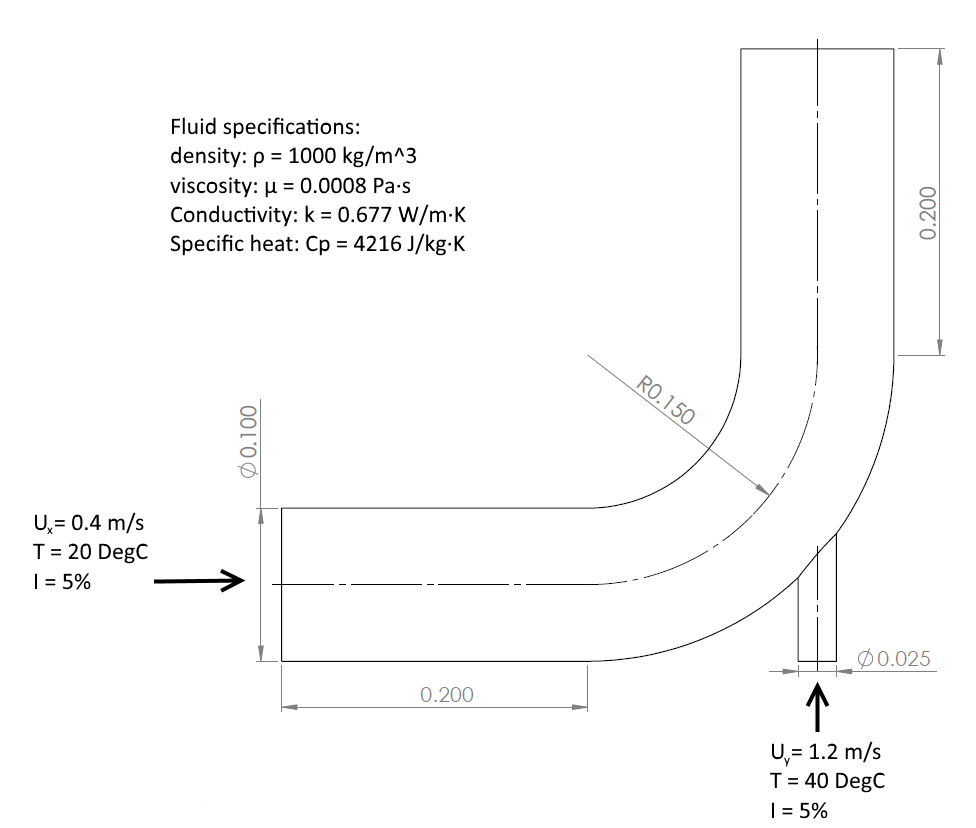
\includegraphics[width=0.95\textwidth,clip]{./Pics/elbow_sketch.png}
\end{center}
\caption{Sketch of the 3D mixing elbow. Dimensions in meters.}\label{Design1:Sketch1}
\end{figure}

%%%
%%% SECTION
%%%
\section{Numerical Simulation}

%%% SUBSECTION
\subsection{Creating the 3D Geometry}
Add a new \bfr{Geometry} component to your \emph{workbench} and ensure that your analysis type is set to \bfr{3D}. Open \bfr{Geometry} and set your units to \bfr{Meter}. Insert a new sketch by clicking  
\includegraphics[width=.4cm]{./Pics/new_sketch.png} in the \bfr{YZPlane}, select 
\includegraphics[width=.4cm]{./Pics/normal_to.png} to obtain a view normal to the sketch plane. Draw an \bfr{Arc by Center} with the centre at the origin and radius of \bfr{5\,cm} as shown below and enclose the ends of the arc with a vertical line. Create a new sketch in the \bfr{XYPlane} and draw a horizontal line from the origin in positive x-direction and a vertical line as shown below. Give each line a dimension of \bfr{35\,cm}.
\begin{figure}[H] 
\begin{center}
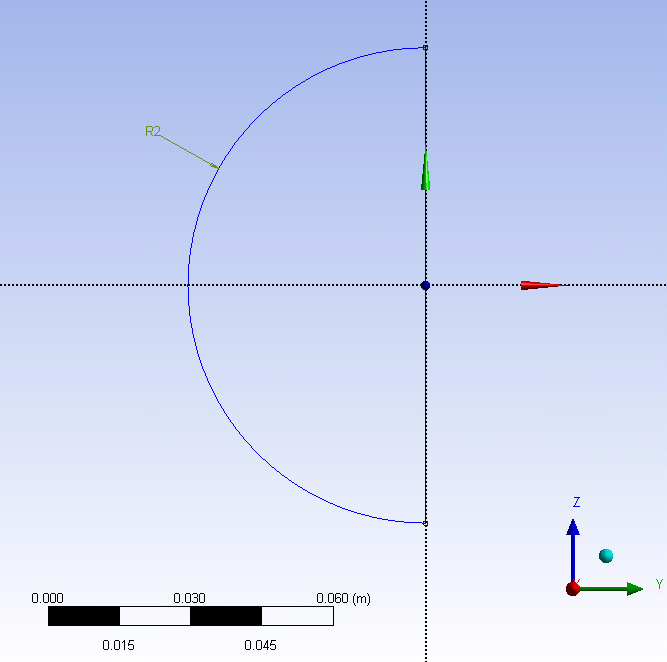
\includegraphics[height=0.4\textwidth,clip]{./Pics/semi_circle.png}\quad
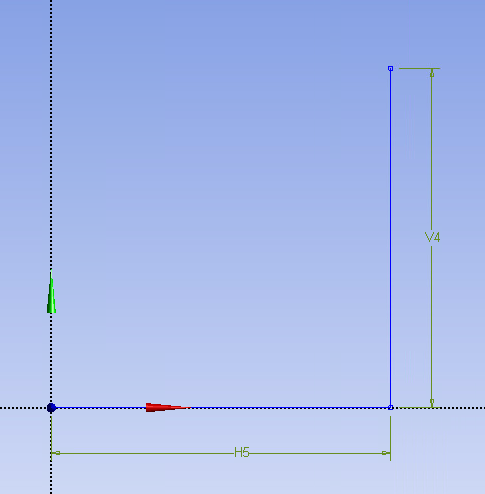
\includegraphics[height=0.4\textwidth,clip]{./Pics/hor_vert_line.png}
\end{center}
\end{figure}
Next apply a fillet to the edge between the horizontal and vertical line, select the \bfr{Modify} menu and select 
\includegraphics[width=1cm]{./Pics/fillet.png}.  Specify a small radius of, say, 0.01\,cm in the radius cell 
\includegraphics[width=2cm]{./Pics/fillet_radius.png}. While holding \bfr{Ctrl} select the horizontal and vertical line, after selecting the vertical line you will see that the fillet is applied. Now use the radius dimensioning tool to set the radius of the fillet to 0.15\,m. Go back to the \bfr{Modeling Tab}, select the sketch in the \emph{Tree Outline}, in the \emph{Details View} change the sketch visibility to \bfr{Always Show Sketch}. Repeat this procedure for the initial sketch you made in the YZPlane. Select 
\includegraphics[width=1.4cm]{./Pics/sweep.png} from the toolbar and in the \emph{Tree Outline} select the sketch you made in the \bfr{YZPlane}, then in the \emph{Details View} click the \bfr{Apply} button - your sketch should now have appeared in the \emph{Profile} box. Now select the yellow \bfr{Not selected} box in the \emph{Path} box and select in the \emph{Tree Outline} the sketch you made in the \bfr{XYPlane} and click \bfr{Apply} in the \emph{Details View}. Click the 
\includegraphics[width=1.4cm]{./Pics/generate_button.png} button to create the pipe elbow.

\bigskip
Create a new plane by clicking 
\includegraphics[width=0.4cm]{./Pics/new_plane.png} in the \emph{Sketch Toolbar}, note how \emph{Plane4} has appeared in the \emph{Tree Outline}. In the details view select the \bfr{XYPlane} in the \emph{Base Plane} option box, select the \bfr{ZXPlane} in the \emph{Tree Outline} and click \bfr{Apply} in the \emph{Details View}. Select \bfr{Offset Y} as the option for \emph{Transform 1 (RMB)}, and apply an offset of \bfr{0.35}\,m as option in the \emph{FD1, Value1} box which has appeared. Using \emph{Transform 1 (RMB)} apply another \bfr{Offset Z} of \bfr{-0.05}\,m. Note how the origin of your newly create plane appears under the centreline of the vertical pipe segment and in the same plane as the bottom of the horizontal pipe segment as shown below. Click 
\includegraphics[width=1.4cm]{./Pics/generate_button.png} to create the plane. Now is a good time to inspect your geometry using the various button in the \emph{rotation mode toolbar}.
\begin{figure}[H]
\begin{center}
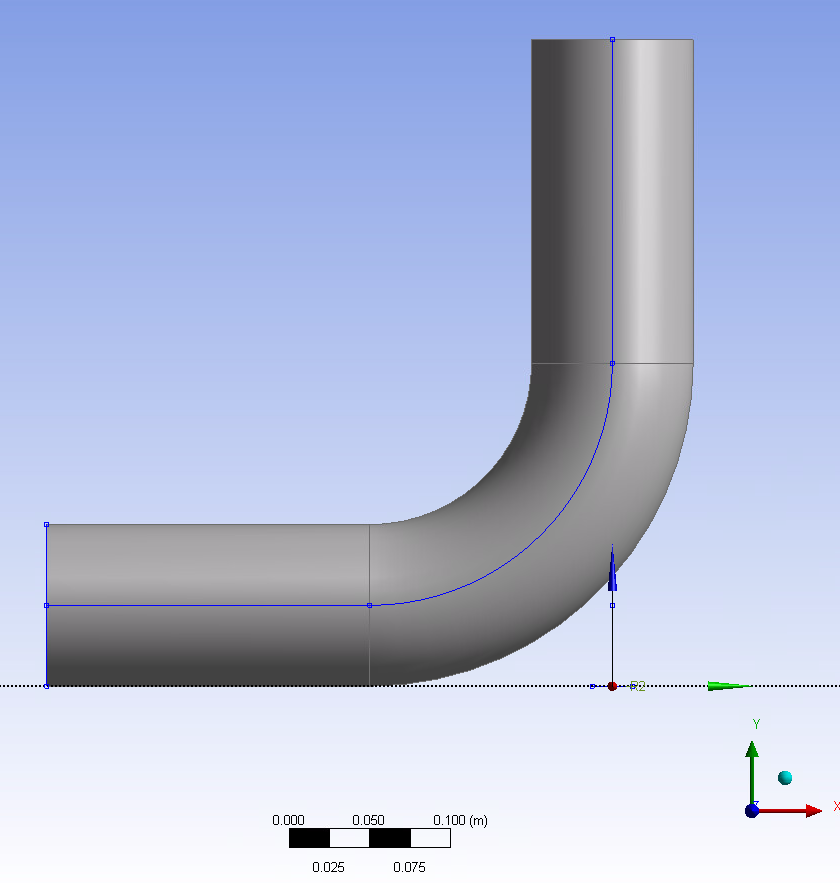
\includegraphics[width=0.6\textwidth,clip]{./Pics/new_plane_origin.png}
\end{center}
\end{figure}
Select your newly created plane in the \emph{Tree Outline} and obtain a view normal to the plane, zoom in if necessary to see the origin of the newly created plane. Draw another enclosed semi-circle with the origin at its center using \bfr{Arc by Center} and give it a radius of \bfr{1.25\,cm}. Obtain an isometric view by selecting 
\includegraphics[width=0.4cm]{./Pics/isometric_view1.png} in the \emph{rotation mode toolbar} or click on 
\includegraphics[width=0.3cm]{./Pics/isometric_view2.png} symbol in the lower right corner of your \emph{Graphics Window}. Use the rotation tools to see where the circle has appeared in relation to your pipe geometry. With the sketch still selected, click 
\includegraphics[width=1.4cm]{./Pics/extrude.png} and select \bfr{Apply} in the \emph{Details View}. Change the \emph{Direction} to \bfr{Normal} and change the \emph{Depth} of the extrusion to \bfr{0.1\,m}. Press 
\includegraphics[width=1.4cm]{./Pics/generate_button.png} to create the extrusion. Use the rotation tools again to inspect the model. \bfr{Save} your project and close the \emph{DesignModeler} window.

%%% SUBSECTION
\subsection{Mesh Generation}
Add the \bfr{Mesh} component to your workbench, connect your created Geometry to this component, and open the \bfr{Meshing} tool. First create five \emph{named selections}; two inlets, one outlet, the pipewall and the symmetry plane. Note that you now have used the face select tool 
\includegraphics[width=0.4cm]{./Pics/select_faces.png} to assign names to the faces. Give sensible names to the inlets and also note that the pipewall consists of 4\,faces and the symmetry plane of 3\,faces.

Click on the \bfr{Mesh} in the \emph{Tree Outline} and note how the \emph{Details window} contains many expandable mesh setting categories, these are called to \emph{Global Mesh Controls}. There are also \emph{Local Mesh Controls} which are accessed by right-clicking the mesh in the \emph{Tree Outline} and selecting insert, or through 
\includegraphics[width=2.4cm]{./Pics/mesh_control.png} in the mesh toolbar. More information about the Mesh Control options can be obtained by accessing the \emph{ANSYS Help}. {\bf We strongly encourage you the look at the \emph{Global Mesh Controls} section as part of the \emph{Meshing User's Guide} in order to understand the various mesh settings that you might require later on.}

\medskip

Change the \emph{Physics Preference} to \bfr{CFD} and ensure that the \emph{Solver Preference} is set to \bfr{Fluent}. Expand the \emph{Sizing} and \emph{Inflation} categories. With the \emph{Sizing} option you control the cell sizes of your mesh in various ways, while \emph{Inflation} allows us to refine the mesh near the walls to capture the near-wall flow more accurately. Right-click on \bfr{Mesh} in the \emph{Tree Outline} and select \bfr{Generate Mesh}. By default a mesh consisting of tetrahedron shaped cells is created (i.e. \emph{Tetrahedral Mesh}). Use the rotation tools to explore your mesh and note the refinement of the mesh in, and near, the small inlet pipe.

\medskip
Under \emph{Sizing} set the \emph{Relevance Centre} to \emph{medium} and also set the \emph{Span Angle Centre} to \emph{Coarse}. Now change \emph{Use Automatic Inflation} to \bfr{All Faces in Chosen Named Selection} and for \emph{Named Selection} choose your \bfr{pipewall} (or whichever name you have assigned to it). Set the \emph{maximum layers} to \bfr{3}, we'll leave the other settings at their default values for now. You can change the \emph{Maximum Layers} to increase the amount of layers near the wall should that be required or alternatively near wall inflation might not be necessary at all in which can you can switch it off. Now in the \bfr{Tree outline} right-click on the Mesh and select \bfr{Update} or \bfr{Generate Mesh}. If you now look at the \emph{Statistics} menu you will see that there are approximately 8500 elements in your mesh. Now under the \emph{Defaults} category use the \emph{Relevance} slider to obtain \emph{approximately} 20k elements. You may need to adjust the slider a few times and re-generate the mesh to obtain an appropriate mesh resolution. Note that you do not need exactly 20k elements a couple of hundred more or less is OK. Inspect the inlets and outlet of your model to check how \emph{Inflation} has impacted on the mesh. The isometric view of your pipe should look as follows:

\begin{figure}[H]
\begin{center}
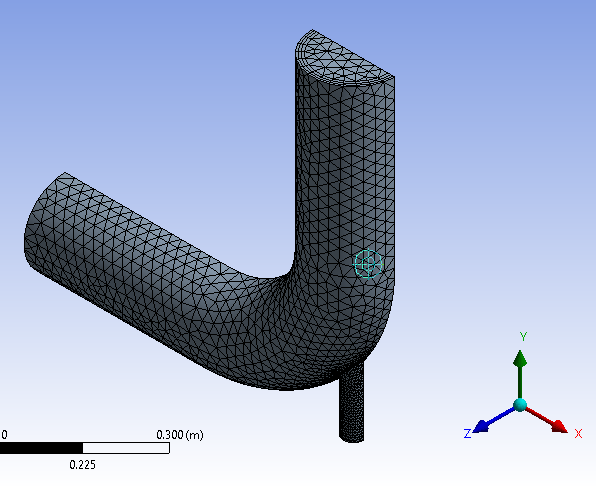
\includegraphics[width=0.6\textwidth,clip]{./Pics/isom_view_pipe.png}
\end{center}
\end{figure}
Close the meshing window and \bfr{save} your project.

%%% SUBSECTION
\subsection{Model Setup}
Now you can set-up the Fluent model and perform the simulation. Setting up Fluent is very similar to what you have done in the previous labs so we will not repeat that here. A couple of things to note:
\begin{itemize}
\item[-] use the $k-\varepsilon$ turbulence model;
\item[-] edit the \emph{Cell Zone Conditions} such that the \emph{Zone Name} is fluid with \emph{Material Name} set the to the fluid which you created in the \emph{Materials} section;
\item[-] in the \emph{solution methods} set the \emph{spatial discretization} to \emph{Second Order Upwind};
\item[-] in the residual monitor set the \emph{Absolute criteria} for continuity, momentum and energy to $10^{-4}$ and for $k$ and epsilon to $10^{-3}$;
\item[-] create a surface monitor, name  it \texttt{outlet\_temp\_avg}, select for \emph{Report Type} the option \emph{Mass-Weighted Average} and select \emph{Temperature...} and \emph{Static Temperature} as Field Variable and select \emph{outlet} as the surface. This will create a monitor for the average outlet temperature. Tick the \emph{Plot} box so that it will be displayed. In the Monitors menu select 
\includegraphics[width=2.4cm]{./Pics/convergence_manager.png}, you will see that \texttt{outlet\_temp\_avg} is available as a convergence monitor. Sicne we are particularly interested in the outlet temperature we will set it as our 8$^\mathrm{th}$ monitor, set the stop criterion to 1e-6, and set the other two options to 15 and 10, respectively;
\item[-] you can use hybrid initialisation or standard initialisation;
\end{itemize}



\section{Tasks}
\subsection{Single Phase Flow Mixing through a 90 Degree Bend}\label{Task:Section1}
 For this first set of numerical simulations, a cold liquid water flows through the main pipeline at 20 $^{\circ}$C $\left(\text{and 0.4 m.s}^{-1}\right)$ and hot liquid water $\left(\text{1.2 m.s}^{-1}\right)$ is injected along the pipe elbow at 40 $^{\circ}$C (see Fig.~\ref{Design1:Sketch1}). Assume that both fluid streams are incompressible and both pipes are fully insulated (i.e., adiabatic or zero heat flux conditions).
    
     
    \begin{shaded}
    Perform simulations with mesh resolutions of (approximately) 20k, 40k and 60k elements. \emph{Plot and compare} the numerical results of the velocity at centreline of the pipe outlet for these mesh grids. We often assume that \emph{solution mesh independence} (also known as \emph{mesh convergence}) is achieved when there is no improvement of the solution (mainly for either velocity or pressure fluctuation fields)  after increasing mesh resolution. In our case, extract (i.e., export)  the values of velocity magnitudes at the centreline of the pipe outlet for the four mesh grids. Using either Matlab or Excel, calculate the error of two sets of velocity magnitude vectors obtained from simulations of two consecutive grid resolutions, 
        \begin{displaymath}
           \mathcal{E} = \frac{\sum\limits_{i=1}^{N}\left(\frac{\left|v_{i}^{(k)}-v_{i}^{(k-1)}\right|}{v_{i}^{(k-1)}}\right)}{N}\times 100\;\;\;\;\left(\%\right)
        \end{displaymath}
        where $v^{(k)}$ is the vector representing the velocity magnitudes at grid resolution $k$ and $N$ is the number of sample points (i.e., length of the velocity magnitude vectors). 
        \medskip
        
        In engineering design problems in which detailed fluid flow dynamics is required, a numerical solution is assumed mesh-independent if $\mathcal{E} \le 0.1\%$. Before we reach the required grid resolution a number of simulations with coarse grids are often performed for testing different aspects of solution methods, thermo-physical properties, boundary conditions etc, towards an optimal design. Here, for the remaining numerical simulations you should use a mesh grid resolution with 60k elements.
        \medskip
        
        In the report, you should include and comment on (based on simulations performed with 60k mesh resolution)
    \begin{enumerate}
        \item Plot $y^{+}\;\times$ {\it x-position} along the pipewall;
        \item Velocity vectors overlapped with temperature contour-plot for the symmetry plane;
        \item Plot temperature $\times$ {\it x-position} at centreline of the pipe outlet;
    \end{enumerate}
    \end{shaded}
    
\subsection{Pre-Heated Mixed System}
Use a similar simulation setup as Section~\ref{Task:Section1} (with mesh resolution of 60k), but now:
    \begin{enumerate}[i)]
       \item Split the horizontal pipe domain before the 90$^{\circ}$ bend into three segments of 5, 10 and 5\,cm, the procedure is similar to the one in the previous practical;
       \item In the second segment ($5\le x \le 15$ cm), impose:
       \begin{itemize}
          \item Case 1: prescribed heat flux boundary condition of 100 kW.m$^{-2}$;
          \item Case 2: prescribed wall temperature of 30$^{\circ}$C;
        \end{itemize}
    \end{enumerate}
    
    \begin{shaded}    
    Repeat the plots highlighted in Section~\ref{Task:Section1} and comment on the differences of:
    \begin{enumerate}
      \item temperature profiles along the symmetry plane;
      \item velocity profiles along the symmetry plane;
      \item temperature profiles at centreline of the pipe outlet.
    \end{enumerate}
    \end{shaded}
    
\clearpage
\begin{center}
\Large{\bf Deliverables}
\end{center}
General instructions for the Final Report (containing parts 1 and 2 of the assignment):
\begin{enumerate}[1)]
\begin{shaded}
\item Part 2 of this Assignment will be released in \emph{MyAberdeen} on November 9$^{\text{th}}$ at noon.
\end{shaded}
  \item Write a report containing:
  \begin{enumerate}
    \item Summary of {\bf all simulation set-ups} including,
       \begin{enumerate} [(a)]
          \item Initial and boundary conditions (for each simulation);
          \item Mesh information/quality;
          \item Numerical schemes (i.e., solution methods) and sub-models used.
       \end{enumerate}
    \item Summary of the numerical results (incl. figures displaying the data -- shaded areas above), findings, interpretation and \underline{analysis} along with concluding remarks.
  \end{enumerate}
  
  \item Report should contain no more than (\underline{maximum}) 25 pages including cover page, bibliography and appendices (if any);

\item {\bf Prepare the report (containing results of Parts 1 and 2 of this assignment) as \underline{PDF file} and submit it through {\it Turnitin} (with the appropriate plagiarism cover sheet) by Friday, November 25$^{\text{th}}$ 2016, noon at the latest. Also, submit a hard-copy of the report to the UG office by November 25$^{\text{th}}$, 15.00h.}
%
%\item Feedback will be provided on December YY$^{th}$ 2015.
%
\item Penalties for late or non-submission are as follows:
\begin{enumerate}%[(a)]
\item Up to one week late, 2 CGS points deducted;
\item Up to two weeks late, 3 CGS point deducted;
\item More than two weeks late no marks awarded.
\end{enumerate}
If late or non-submission is due to medical or other circumstances out with your control you must submit a medical certificate or other formal evidence to the UG Office as soon as is practicable but no later than the end of Revision Week.


\item Note that the submitted work is part of the continuous assessment which will contribute 40$\%$ to your EG501V mark.

\end{enumerate}

\end{document}
